% Created by tikzDevice version 0.12.6 on 2025-04-07 02:23:31
% !TEX encoding = UTF-8 Unicode
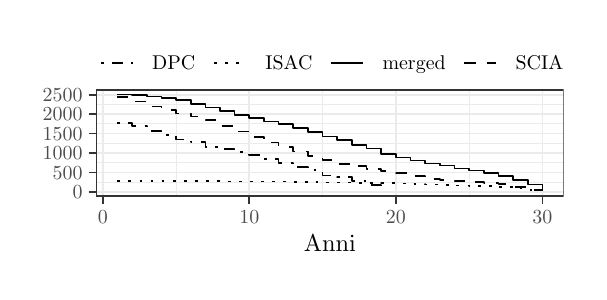
\begin{tikzpicture}[x=1pt,y=1pt]
\definecolor{fillColor}{RGB}{255,255,255}
\path[use as bounding box,fill=fillColor] (0,0) rectangle (199.17, 88.20);
\begin{scope}
\path[clip] (  0.00,  0.00) rectangle (199.17, 88.20);
\definecolor{drawColor}{RGB}{255,255,255}

\path[draw=drawColor,line width= 0.6pt,line join=round,line cap=round,fill=fillColor] (  0.00,  0.00) rectangle (199.17, 88.20);
\end{scope}
\begin{scope}
\path[clip] ( 24.75, 27.29) rectangle (193.67, 65.79);
\definecolor{fillColor}{RGB}{255,255,255}

\path[fill=fillColor] ( 24.75, 27.29) rectangle (193.67, 65.79);
\definecolor{drawColor}{gray}{0.92}

\path[draw=drawColor,line width= 0.3pt,line join=round] ( 24.75, 32.33) --
	(193.67, 32.33);

\path[draw=drawColor,line width= 0.3pt,line join=round] ( 24.75, 39.36) --
	(193.67, 39.36);

\path[draw=drawColor,line width= 0.3pt,line join=round] ( 24.75, 46.40) --
	(193.67, 46.40);

\path[draw=drawColor,line width= 0.3pt,line join=round] ( 24.75, 53.43) --
	(193.67, 53.43);

\path[draw=drawColor,line width= 0.3pt,line join=round] ( 24.75, 60.46) --
	(193.67, 60.46);

\path[draw=drawColor,line width= 0.3pt,line join=round] ( 53.61, 27.29) --
	( 53.61, 65.79);

\path[draw=drawColor,line width= 0.3pt,line join=round] (106.56, 27.29) --
	(106.56, 65.79);

\path[draw=drawColor,line width= 0.3pt,line join=round] (159.51, 27.29) --
	(159.51, 65.79);

\path[draw=drawColor,line width= 0.6pt,line join=round] ( 24.75, 28.81) --
	(193.67, 28.81);

\path[draw=drawColor,line width= 0.6pt,line join=round] ( 24.75, 35.85) --
	(193.67, 35.85);

\path[draw=drawColor,line width= 0.6pt,line join=round] ( 24.75, 42.88) --
	(193.67, 42.88);

\path[draw=drawColor,line width= 0.6pt,line join=round] ( 24.75, 49.91) --
	(193.67, 49.91);

\path[draw=drawColor,line width= 0.6pt,line join=round] ( 24.75, 56.95) --
	(193.67, 56.95);

\path[draw=drawColor,line width= 0.6pt,line join=round] ( 24.75, 63.98) --
	(193.67, 63.98);

\path[draw=drawColor,line width= 0.6pt,line join=round] ( 27.13, 27.29) --
	( 27.13, 65.79);

\path[draw=drawColor,line width= 0.6pt,line join=round] ( 80.09, 27.29) --
	( 80.09, 65.79);

\path[draw=drawColor,line width= 0.6pt,line join=round] (133.04, 27.29) --
	(133.04, 65.79);

\path[draw=drawColor,line width= 0.6pt,line join=round] (185.99, 27.29) --
	(185.99, 65.79);
\definecolor{drawColor}{RGB}{0,0,0}

\path[draw=drawColor,line width= 0.6pt,dash pattern=on 1pt off 3pt on 4pt off 3pt ,line join=round] ( 32.43, 53.80) --
	( 37.72, 53.80) --
	( 37.72, 52.61) --
	( 43.02, 52.61) --
	( 43.02, 50.93) --
	( 48.31, 50.93) --
	( 48.31, 49.34) --
	( 53.61, 49.34) --
	( 53.61, 47.73) --
	( 58.90, 47.73) --
	( 58.90, 46.83) --
	( 64.20, 46.83) --
	( 64.20, 45.06) --
	( 69.50, 45.06) --
	( 69.50, 44.46) --
	( 74.79, 44.46) --
	( 74.79, 43.19) --
	( 80.09, 43.19) --
	( 80.09, 42.15) --
	( 85.38, 42.15) --
	( 85.38, 40.83) --
	( 90.68, 40.83) --
	( 90.68, 39.35) --
	( 95.97, 39.35) --
	( 95.97, 37.77) --
	(101.27, 37.77) --
	(101.27, 36.69) --
	(106.56, 36.69) --
	(106.56, 34.83) --
	(111.86, 34.83) --
	(111.86, 34.22) --
	(117.15, 34.22) --
	(117.15, 32.77) --
	(122.45, 32.77) --
	(122.45, 31.37) --
	(127.74, 31.37) --
	(127.74, 29.53);

\path[draw=drawColor,line width= 0.6pt,dash pattern=on 1pt off 3pt ,line join=round] ( 32.43, 32.72) --
	( 37.72, 32.72) --
	( 37.72, 32.72) --
	( 43.02, 32.72) --
	( 43.02, 32.72) --
	( 48.31, 32.72) --
	( 48.31, 32.72) --
	( 53.61, 32.72) --
	( 53.61, 32.72) --
	( 58.90, 32.72) --
	( 58.90, 32.70) --
	( 64.20, 32.70) --
	( 64.20, 32.68) --
	( 69.50, 32.68) --
	( 69.50, 32.65) --
	( 74.79, 32.65) --
	( 74.79, 32.63) --
	( 80.09, 32.63) --
	( 80.09, 32.63) --
	( 85.38, 32.63) --
	( 85.38, 32.60) --
	( 90.68, 32.60) --
	( 90.68, 32.57) --
	( 95.97, 32.57) --
	( 95.97, 32.48) --
	(101.27, 32.48) --
	(101.27, 32.36) --
	(106.56, 32.36) --
	(106.56, 32.26) --
	(111.86, 32.26) --
	(111.86, 32.20) --
	(117.15, 32.20) --
	(117.15, 32.16) --
	(122.45, 32.16) --
	(122.45, 32.12) --
	(127.74, 32.12) --
	(127.74, 32.01) --
	(133.04, 32.01) --
	(133.04, 31.92) --
	(138.33, 31.92) --
	(138.33, 31.75) --
	(143.63, 31.75) --
	(143.63, 31.58) --
	(148.92, 31.58) --
	(148.92, 31.44) --
	(154.22, 31.44) --
	(154.22, 31.22) --
	(159.51, 31.22) --
	(159.51, 31.09) --
	(164.81, 31.09) --
	(164.81, 30.92) --
	(170.11, 30.92) --
	(170.11, 30.56) --
	(175.40, 30.56) --
	(175.40, 30.09) --
	(180.70, 30.09) --
	(180.70, 29.66) --
	(185.99, 29.66) --
	(185.99, 29.04);

\path[draw=drawColor,line width= 0.6pt,line join=round] ( 32.43, 64.04) --
	( 37.72, 64.04) --
	( 37.72, 63.94) --
	( 43.02, 63.94) --
	( 43.02, 63.39) --
	( 48.31, 63.39) --
	( 48.31, 62.74) --
	( 53.61, 62.74) --
	( 53.61, 62.01) --
	( 58.90, 62.01) --
	( 58.90, 60.72) --
	( 64.20, 60.72) --
	( 64.20, 59.34) --
	( 69.50, 59.34) --
	( 69.50, 58.04) --
	( 74.79, 58.04) --
	( 74.79, 56.64) --
	( 80.09, 56.64) --
	( 80.09, 55.48) --
	( 85.38, 55.48) --
	( 85.38, 54.29) --
	( 90.68, 54.29) --
	( 90.68, 53.29) --
	( 95.97, 53.29) --
	( 95.97, 51.95) --
	(101.27, 51.95) --
	(101.27, 50.46) --
	(106.56, 50.46) --
	(106.56, 48.90) --
	(111.86, 48.90) --
	(111.86, 47.54) --
	(117.15, 47.54) --
	(117.15, 45.85) --
	(122.45, 45.85) --
	(122.45, 44.50) --
	(127.74, 44.50) --
	(127.74, 42.65) --
	(133.04, 42.65) --
	(133.04, 41.26) --
	(138.33, 41.26) --
	(138.33, 40.24) --
	(143.63, 40.24) --
	(143.63, 39.11) --
	(148.92, 39.11) --
	(148.92, 38.35) --
	(154.22, 38.35) --
	(154.22, 37.28) --
	(159.51, 37.28) --
	(159.51, 36.59) --
	(164.81, 36.59) --
	(164.81, 35.62) --
	(170.11, 35.62) --
	(170.11, 34.57) --
	(175.40, 34.57) --
	(175.40, 33.24) --
	(180.70, 33.24) --
	(180.70, 31.50) --
	(185.99, 31.50) --
	(185.99, 29.63);

\path[draw=drawColor,line width= 0.6pt,dash pattern=on 4pt off 4pt ,line join=round] ( 32.43, 63.12) --
	( 37.72, 63.12) --
	( 37.72, 61.49) --
	( 43.02, 61.49) --
	( 43.02, 59.76) --
	( 48.31, 59.76) --
	( 48.31, 58.47) --
	( 53.61, 58.47) --
	( 53.61, 57.24) --
	( 58.90, 57.24) --
	( 58.90, 56.16) --
	( 64.20, 56.16) --
	( 64.20, 54.88) --
	( 69.50, 54.88) --
	( 69.50, 52.74) --
	( 74.79, 52.74) --
	( 74.79, 50.64) --
	( 80.09, 50.64) --
	( 80.09, 48.60) --
	( 85.38, 48.60) --
	( 85.38, 46.68) --
	( 90.68, 46.68) --
	( 90.68, 45.17) --
	( 95.97, 45.17) --
	( 95.97, 43.44) --
	(101.27, 43.44) --
	(101.27, 41.91) --
	(106.56, 41.91) --
	(106.56, 40.50) --
	(111.86, 40.50) --
	(111.86, 39.04) --
	(117.15, 39.04) --
	(117.15, 38.11) --
	(122.45, 38.11) --
	(122.45, 37.21) --
	(127.74, 37.21) --
	(127.74, 36.31) --
	(133.04, 36.31) --
	(133.04, 35.62) --
	(138.33, 35.62) --
	(138.33, 34.65) --
	(143.63, 34.65) --
	(143.63, 33.50) --
	(148.92, 33.50) --
	(148.92, 33.16) --
	(154.22, 33.16) --
	(154.22, 32.70) --
	(159.51, 32.70) --
	(159.51, 32.34) --
	(164.81, 32.34) --
	(164.81, 32.05) --
	(170.11, 32.05) --
	(170.11, 31.63) --
	(175.40, 31.63) --
	(175.40, 30.61) --
	(180.70, 30.61) --
	(180.70, 29.47) --
	(185.99, 29.47) --
	(185.99, 29.07);
\definecolor{drawColor}{gray}{0.20}

\path[draw=drawColor,line width= 0.6pt,line join=round,line cap=round] ( 24.75, 27.29) rectangle (193.67, 65.79);
\end{scope}
\begin{scope}
\path[clip] (  0.00,  0.00) rectangle (199.17, 88.20);
\definecolor{drawColor}{gray}{0.30}

\node[text=drawColor,anchor=base east,inner sep=0pt, outer sep=0pt, scale=  0.72] at ( 19.80, 26.35) {0};

\node[text=drawColor,anchor=base east,inner sep=0pt, outer sep=0pt, scale=  0.72] at ( 19.80, 33.38) {500};

\node[text=drawColor,anchor=base east,inner sep=0pt, outer sep=0pt, scale=  0.72] at ( 19.80, 40.42) {1000};

\node[text=drawColor,anchor=base east,inner sep=0pt, outer sep=0pt, scale=  0.72] at ( 19.80, 47.45) {1500};

\node[text=drawColor,anchor=base east,inner sep=0pt, outer sep=0pt, scale=  0.72] at ( 19.80, 54.48) {2000};

\node[text=drawColor,anchor=base east,inner sep=0pt, outer sep=0pt, scale=  0.72] at ( 19.80, 61.52) {2500};
\end{scope}
\begin{scope}
\path[clip] (  0.00,  0.00) rectangle (199.17, 88.20);
\definecolor{drawColor}{gray}{0.20}

\path[draw=drawColor,line width= 0.6pt,line join=round] ( 22.00, 28.81) --
	( 24.75, 28.81);

\path[draw=drawColor,line width= 0.6pt,line join=round] ( 22.00, 35.85) --
	( 24.75, 35.85);

\path[draw=drawColor,line width= 0.6pt,line join=round] ( 22.00, 42.88) --
	( 24.75, 42.88);

\path[draw=drawColor,line width= 0.6pt,line join=round] ( 22.00, 49.91) --
	( 24.75, 49.91);

\path[draw=drawColor,line width= 0.6pt,line join=round] ( 22.00, 56.95) --
	( 24.75, 56.95);

\path[draw=drawColor,line width= 0.6pt,line join=round] ( 22.00, 63.98) --
	( 24.75, 63.98);
\end{scope}
\begin{scope}
\path[clip] (  0.00,  0.00) rectangle (199.17, 88.20);
\definecolor{drawColor}{gray}{0.20}

\path[draw=drawColor,line width= 0.6pt,line join=round] ( 27.13, 24.54) --
	( 27.13, 27.29);

\path[draw=drawColor,line width= 0.6pt,line join=round] ( 80.09, 24.54) --
	( 80.09, 27.29);

\path[draw=drawColor,line width= 0.6pt,line join=round] (133.04, 24.54) --
	(133.04, 27.29);

\path[draw=drawColor,line width= 0.6pt,line join=round] (185.99, 24.54) --
	(185.99, 27.29);
\end{scope}
\begin{scope}
\path[clip] (  0.00,  0.00) rectangle (199.17, 88.20);
\definecolor{drawColor}{gray}{0.30}

\node[text=drawColor,anchor=base,inner sep=0pt, outer sep=0pt, scale=  0.72] at ( 27.13, 17.41) {0};

\node[text=drawColor,anchor=base,inner sep=0pt, outer sep=0pt, scale=  0.72] at ( 80.09, 17.41) {10};

\node[text=drawColor,anchor=base,inner sep=0pt, outer sep=0pt, scale=  0.72] at (133.04, 17.41) {20};

\node[text=drawColor,anchor=base,inner sep=0pt, outer sep=0pt, scale=  0.72] at (185.99, 17.41) {30};
\end{scope}
\begin{scope}
\path[clip] (  0.00,  0.00) rectangle (199.17, 88.20);
\definecolor{drawColor}{RGB}{0,0,0}

\node[text=drawColor,anchor=base,inner sep=0pt, outer sep=0pt, scale=  0.88] at (109.21,  7.21) {Anni};
\end{scope}
\begin{scope}
\path[clip] (  0.00,  0.00) rectangle (199.17, 88.20);
\definecolor{fillColor}{RGB}{255,255,255}

\path[fill=fillColor] ( 24.99, 76.79) rectangle (193.42, 82.70);
\end{scope}
\begin{scope}
\path[clip] (  0.00,  0.00) rectangle (199.17, 88.20);
\definecolor{fillColor}{RGB}{255,255,255}

\path[fill=fillColor] ( 24.99, 68.25) rectangle ( 39.45, 82.70);
\end{scope}
\begin{scope}
\path[clip] (  0.00,  0.00) rectangle (199.17, 88.20);
\definecolor{drawColor}{RGB}{0,0,0}

\path[draw=drawColor,line width= 0.6pt,dash pattern=on 1pt off 3pt on 4pt off 3pt ,line join=round] ( 26.44, 75.48) -- ( 38.00, 75.48);
\end{scope}
\begin{scope}
\path[clip] (  0.00,  0.00) rectangle (199.17, 88.20);
\definecolor{fillColor}{RGB}{255,255,255}

\path[fill=fillColor] ( 65.94, 68.25) rectangle ( 80.39, 82.70);
\end{scope}
\begin{scope}
\path[clip] (  0.00,  0.00) rectangle (199.17, 88.20);
\definecolor{drawColor}{RGB}{0,0,0}

\path[draw=drawColor,line width= 0.6pt,dash pattern=on 1pt off 3pt ,line join=round] ( 67.39, 75.48) -- ( 78.95, 75.48);
\end{scope}
\begin{scope}
\path[clip] (  0.00,  0.00) rectangle (199.17, 88.20);
\definecolor{fillColor}{RGB}{255,255,255}

\path[fill=fillColor] (108.28, 68.25) rectangle (122.73, 82.70);
\end{scope}
\begin{scope}
\path[clip] (  0.00,  0.00) rectangle (199.17, 88.20);
\definecolor{drawColor}{RGB}{0,0,0}

\path[draw=drawColor,line width= 0.6pt,line join=round] (109.72, 75.48) -- (121.28, 75.48);
\end{scope}
\begin{scope}
\path[clip] (  0.00,  0.00) rectangle (199.17, 88.20);
\definecolor{fillColor}{RGB}{255,255,255}

\path[fill=fillColor] (156.39, 68.25) rectangle (170.84, 82.70);
\end{scope}
\begin{scope}
\path[clip] (  0.00,  0.00) rectangle (199.17, 88.20);
\definecolor{drawColor}{RGB}{0,0,0}

\path[draw=drawColor,line width= 0.6pt,dash pattern=on 4pt off 4pt ,line join=round] (157.84, 75.48) -- (169.40, 75.48);
\end{scope}
\begin{scope}
\path[clip] (  0.00,  0.00) rectangle (199.17, 88.20);
\definecolor{drawColor}{RGB}{0,0,0}

\node[text=drawColor,anchor=base west,inner sep=0pt, outer sep=0pt, scale=  0.72] at ( 44.95, 73.01) {DPC};
\end{scope}
\begin{scope}
\path[clip] (  0.00,  0.00) rectangle (199.17, 88.20);
\definecolor{drawColor}{RGB}{0,0,0}

\node[text=drawColor,anchor=base west,inner sep=0pt, outer sep=0pt, scale=  0.72] at ( 85.89, 73.01) {ISAC};
\end{scope}
\begin{scope}
\path[clip] (  0.00,  0.00) rectangle (199.17, 88.20);
\definecolor{drawColor}{RGB}{0,0,0}

\node[text=drawColor,anchor=base west,inner sep=0pt, outer sep=0pt, scale=  0.72] at (128.23, 73.01) {merged};
\end{scope}
\begin{scope}
\path[clip] (  0.00,  0.00) rectangle (199.17, 88.20);
\definecolor{drawColor}{RGB}{0,0,0}

\node[text=drawColor,anchor=base west,inner sep=0pt, outer sep=0pt, scale=  0.72] at (176.34, 73.01) {SCIA};
\end{scope}
\end{tikzpicture}
